%%%%%%%%%%%%%%%%%%%%%%%%%%%%%%%%%%%%%%%%%%
 %Copyright (C) 2018-2020 YuZJ.
%使用CC-BY-NC-SA授权。一份完整版本的许可证已位于附录。这个版本原始作者YuZJ,
%邮箱theafamily@126.com(最后连接于2019年06月20日17:32:17)。
%%%%%%%%%%%%%%%%%%%%%%%%%%%%%%%%%%%%%%%%%%
\part{开始之前}
\chapter*{版权}
版权所有\copyright{} 2018-2020 YuZJ. \par
使用CC-BY-NC-SA授权。一份完整版本的许可证已位于附录。这个版本原始作者YuZJ,邮箱\url{theafamily@126.com}(最后连接于2020年3月29日22:47:08)。\par
本书使用了Adobe公司提供的相关字体。包括:
\begin{verbatim}
SourceHanSansSC-Bold.otf
SourceHanSansSC-Regular.otf
SourceHanSerifSC-Bold.otf
SourceHanSerifSC-Regular.otf
\end{verbatim}
字体对应的许可证已经附于附录。
\begin{center}
{\large \bf\color{red}对本文档所引起的任何后果不作担保!}
\end{center}
\chapter{序言}
《天工开物·序言》描述当时人们在生产方面的创造时写道:“天覆地载,物号数万,而事亦因之,曲成而不遗。”人类在计算机技术上的创造亦是如此。很高兴生活在信息技术快速发展的新时代,国内外优秀的软件都可以被获取以为我们所用。然而“工欲善其事,必先利其器”,对于我们来说,掌握如何高效率地使用计算机是十分重要的。因此,为了方便信息化教学的开展,我结合自己的工作经历,不自量力“年来著书一种”,为希望掌握关于如何高效地使用教室计算机的初级和高级技巧的电教委员或者其余希望提高计算机技能的教师、学生及其他教职人员编写了这份文件。\par
手册中题为“基础:计算机系统”的部分是针对初学者的,它大致介绍了计算机的硬件及软件构成。“使用视窗操作系统实现教学任务”介绍了Windows操作系统的简单技巧与最基础的Windows安全。题为“GNU/Linux的教学实现”的部分是针对已有一定技能基础并希望尝试更加有效的Windows安全工具(如使用以GNU/Linux\footnote{对于“GNU/Linux”操作系统的称法,本书为了保持通用性而决定使用“GNU/Linux”\cite{Why-GNULinux}。关于GNU/Linux的详细介绍参见\pageref{sec:gnulinux}页\ref{sec:gnulinux}。}为操作系统的反病毒光盘清除计算机病毒)并简单地介绍了GNU/Linux 操作系统的入门知识及其教学实现。在介绍多种多样的软件时,我遵循的原则是合法性——性能——易用性——价格。在性能相同的情况下,易用性优先。但我也不会忘了推荐一些不错的自由免费软件以减少希望廉价使用正版软件者的开支。\par
在使用这份手册时,最重要的是实践。本人才疏学浅,请广大读者不吝赐教。如果文档中存在任何侵权之处,请按邮箱联系。一经确认,将立刻改正。希望在选考中取得优良成绩的“大业文人”,应将本书“弃置案头”。“此书于功名进取,毫不相关也。”\par
\begin{flushright}
时己亥年肆月廿七日,西历2019年5月1日\\
慈溪YuZJ于家之书房
\end{flushright}\par
这是电教委员(不)完全技术指南第二版。我们对第一版中的内容进行了修订,更改了某些表述方式以及过时的内容。
\chapter*{预先警告}
\begin{enumerate}
\item 本书内所有网络链接在“最后连接时间”前均有效且已经过Norton Safe Web的Edge插件、Microsoft SmartScreen筛选器及Avira Free Antivirus检测。 
\item 注意,本书中提到的所有应用程序都应该从其官方网站或镜像源处下载。从任何非官方软件发布处(如腾讯电脑管家“软件中心”)下载任何本书中提到的软件是不被推荐的。\par 
\item 从任何网站下载“破解版”或“注册机”“算号器(KeyGen)”“KMS注册机(仅指非法的KMS服务器)”都是不被推荐的。这些程序可能含有“后门”或直接携带病毒(网络蠕虫(Worm)、特洛伊木马(Trojan)和提权程序(Rootkit)\cite{HR1,HR2,HR3,HR4,HR5})。\par
如果你确信你的下载站提供了可靠的软件,你需要使用哈希校验来确保文件可靠性。使用7Zip在文件资源管理器中的右键菜单“CRC SHA”选项校验哈希值并于官方提供的哈希值作比较。如果一致,那么这个软件可被视为是官方的。
\item 请在安装任何软件时查看最终用户许可声明(EULA)和隐私协议。这么将能让你避免一些不必要的麻烦。
\end{enumerate}
经检测的镜像站列表如下(检测于2020年3月29日22:59:54):
\begin{enumerate}
	\item 清华大学开源软件镜像站 \url{https://mirrors.tuna.tsinghua.edu.cn/}
	\item USTC Open Source Software Mirror \url{http://mirrors.ustc.edu.cn/}
	\item 网易开源镜像站 \url{http://ubuntu.cn99.com/},\url{http://mirrors.163.com/}
	\item 华为开源镜像站 \url{https://mirrors.huaweicloud.com/}
	\item 阿里巴巴开源镜像站区 \url{https://developer.aliyun.com/mirror/}
	\item 兰州大学开源社区镜像站 \url{http://mirror.lzu.edu.cn/}
	\item SourceForge \url{https://sourceforge.net/}
	\item FOSSHUB \url{https://www.fosshub.com/}
	\item GitHub \url{https://github.com/}
\end{enumerate}
\chapter{自由软件、开源软件和专有软件}
我们以是否公开源代码\footnote{如果要知道更多关于源代码的信息,请参见\pageref{sec:exe}页的\ref{sec:exe}}为标准来区分一个软件是不是专有软件。不公开源代码的软件被称为专有软件,而公开源代码的软件称为开源或者自由软件。安装时,大部分软件会展示许可证(图像\ref{Fig:FileZillaGPL}),你应该仔细地阅读它并决定是否安装。
\begin{figure}[h]
\centering
	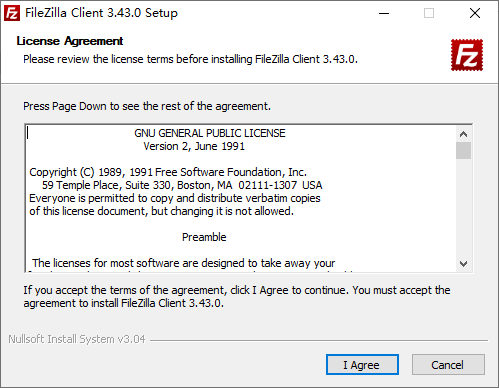
\includegraphics[width=0.7\linewidth]{pic/fzi}
	\caption{安装Filezilla时展示的GNU GPL许可证}
	\label{Fig:FileZillaGPL}
\end{figure}
源代码允许用户“自由”使用的软件称为自由软件。然而,因为“自由”是一个很难定义的名词,因此我们使用Richard Stallman的标准界定“自由”\cite{Whats-Free-Software}。请参见【Various Licenses and Comments about Them - GNU Project - Free Software Foundation】\url{http://www.gnu.org/licenses/license-list.html}(最后连接于2019年07月30日18:08:02)来确定你的许可证是否自由。\par
不同于自由软件的狂热者,我虽然支持自由软件,但是承认拥有\textbf{合法版权}的专有软件的合法性。在这本书中,在\textbf{不影响使用}的前提下如果能完成此功能的专有软件能被自由/开源软件替代,将使用后者。以下是一些常见问题的解答。
\section{使用自由/开源软件有什么好处?}
价格。虽然任何软件的创造者都有权利因自己的创造得到物质上与精神上的回报,但对于消费者来说,自由软件大多数是免费的,但功能强大的专有软件大部分收费。\par
安全性。既然自由/开源软件既然敢于将代码和开发过程示人,就说明他们有勇气接受全世界软件开发者和用户的监督。专有软件的代码不开放性决定了恶意代码或“后门”能被置入代码中。比如,一小部分专有软件会收集大大超过需求的个人信息。\par
维护。自由软件的开发是分布式的。对于活跃的开发社区,大多数漏洞都能在其扩散之前之前被分布在全世界的程序员修补。专有软件和开源软件大多由一家公司开发,任何问题大多数情况下只能依靠公司解决。
\section{为什么自由/开源软件还不流行?}
自由软件在宣传上显然弱于专有软件。使用上,自由软件相较于能实现相同功能的专有软件操作一般较为繁琐(如下图的公式是通过
\begin{verbatim}
	\[-\frac{1}{2 \sigma^2}\left[\sum_{i=1}^n(x_i-\mu_1)^2+\sum_{j=1}^m(y_j-\mu_2)^2\right]\]
\end{verbatim}
\LaTeX 代码生成的,这使自由软件的使用者局限于专业领域从业人员而不是大众。
\begin{figure}[h]
\centering
\fbox{\parbox{6cm}{\[-\frac{1}{2 \sigma^2}\left[\sum_{i=1}^n(x_i-\mu_1)^2+\sum_{j=1}^m(y_j-\mu_2)^2\right]\]}}
\caption{使用\LaTeX 排版公式}
\end{figure}